\chapter{\textcolor{orange}{ADD - ARCHITECTURAL DESIGN DOCUMENT}}
\newpage
\section{\textcolor{orange}{Historial de Versiones}}
\begin{table}[!h]
\begin{center}
\begin{tabular}{|c|c|c|c|}
\hline
\rowcolor[RGB]{255,127,0} Vesión & Fecha & Descripción de Cambios & Autor\\
\hline
1.0 & 15/09/2013 & Primera Versión & Lovaisa V.\\
\hline
\end{tabular}
\end{center}
\end{table}
\newpage

\section{\textcolor{orange}{Página de Aprobaciones}}
A continuación se listan las personas de las cuales se requiere la aceptación de
cualquier cambio mayor de este documento.
\begin{enumerate}
  \item Estas aprobaciones no son necesarias si el cambio es menor.
  \item Estas aprobaciones son necesarias si el cambio es realizado por alguna
  persona distinta de ellas.
\end{enumerate}
\begin{table}[!h]
\begin{center}
\begin{tabular}{|c|c|c|c|}
\hline
\rowcolor[RGB]{255,127,0} Nombre & Cargo & Fecha & Firma\\
\hline
Lovaisa Valeria & Resp. Diseño Arquitectónico & 15/09/2013 & \\
\hline
Gomez Pablo & Resp. Suplente & 15/09/2013 & \\
\hline
\end{tabular}
\end{center}
\end{table}

\newpage
\section{\textcolor{orange}{Introducción}}
\subsection{\textcolor{orange}{Propósito y Alcance}}
Este documento cubre el diseño de la arquitectura  del sistema
de monitoreo y registro de datos multipropósito. Este ADD tiene como objetivo
esteblecer la arquitectura del sistema , sus componentes , patrones
arquitéctonicos utilizados para luego ser implementados en la etapa de desarrollo.

\subsection{\textcolor{orange}{Acrónimos y Glosario}}
\begin{table}[!h]
\begin{center}
\begin{tabular}{|c|c|}
\hline
\rowcolor[RGB]{255,127,0} Acrónimo & Descripción \\
\hline
ADD & Architectural Design Document – Documento de diseño de arquitectura\\
\hline
ADM & Architectural Design Manager – Responsable de diseño de arquitectura\\
\hline
MVC & Model view controller – Modelo vista controlador (Patrón de
Arquitectura)\\
\hline
\end{tabular}
\end{center}
\end{table}

\subsection{\textcolor{orange}{Herramientas Necesarios}}
\begin{table}[!h]
\begin{center}
\begin{tabular}{|c|p{100mm}|}
\hline
\rowcolor[RGB]{255,127,0} Programa & Propósito \\
\hline
Dia & Software para la creación de diagramas UML \\
\hline
\end{tabular}
\end{center}
\end{table}

\newpage
\section{\textcolor{orange}{Roles}}
\subsection{\textcolor{orange}{Responsables}}
Las actividades de ingeniería de requerimientos del Sistema serán coordinadas en
este proyecto por el Responsable de Requerimientos del sistema. (SRM). Este Rol
debe ser asignado a alguno de los miembros del proyecto.
El SRM será el responsable directo de las actividades de requerimientos del
sistema, responder ante modificaciones en los mismos  y de mantener la
documentación relacionada actualizada (Modificación de requerimientos , Matriz
de Trazabilidad , Modificación del sistema de trackeo).


\subsection{\textcolor{orange}{Roles}}
\begin{table}[!h]
\begin{center}
\begin{tabular}{|c|c|c|}
\hline
\rowcolor[RGB]{255,127,0} Rol & Nombre & Suplente\\
\hline
ADM & Lovaisa Valeria & Gomez Pablo\\
\hline
\end{tabular}
\end{center}
\end{table}

\newpage
\section{\textcolor{orange}{Diseño Preliminar}}
\subsection{\textcolor{orange}{Diagrama Preliminar de Diseño de Arquitectura}}
\begin{figure}[h!]
 \begin{center}
  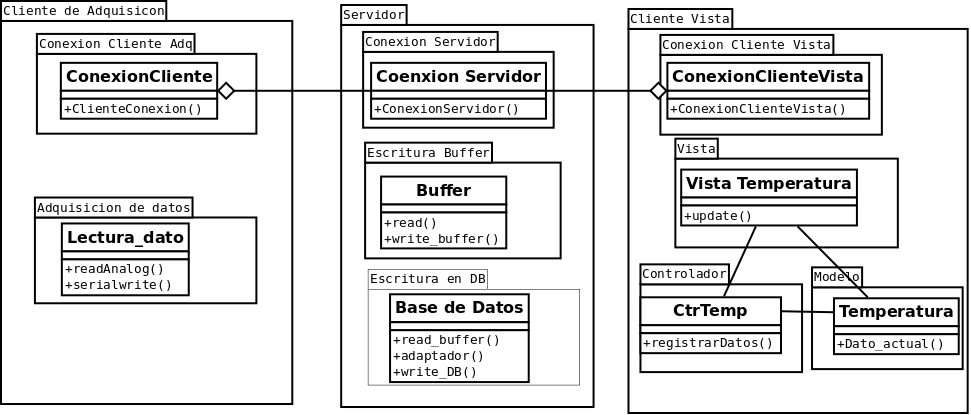
\includegraphics[width=1\textwidth,keepaspectratio=true]{./img/arqprelim.png}
  \caption{Arquitectura Preliminar}
  \label{fig:esquema}
 \end{center}
\end{figure}

\subsection{\textcolor{orange}{Descripción de la Arquitectura Preliminar}}
Se seleccionó el patrón Cliente–Servidor para atacar el modelo de conexión de
los dispositivos de adquision al servidor del sistema. El servidor será el
encargado de correr las instancias necesarias para atender a cada dispositivo
de aquisición conectado via sockets mediante el protocolo UDP.

El servidor es un Iterator, el cual recibe información de cada uno de los
clientes de adquisión e informa a cada uno de los clientes de presentación los
cambios en el modelo (temperaturas , modificación de alarmas , etc).
Con respecto al cliente Presentación , se tiene una arquitectura MVC
(modelo-vista-controlador) donde se encapsulan los datos  de
temperatura (generados por patrón Observer) en el “Modelo” , mientras que el
modelo gráfico se representa en la “Vista” que posee componentes generados
también con el patrón Observer. Finalmente “Vista” presenta , son atendidas por
los objetos contenidos en el paquete “Controlador” cuyas clases componentes son
generadas con el patrón Observer.

Con la aplicación de esta arquitectura se resuelven los requisitos no funciones
relacionados a las diferentes formas de interactuar con los datos.
Permite vez lograr aplicar sin mayores cambios futuros requerimientos para la
interacción y presentación de los datos.

Respecto al modelo Cliente – Servidor aplicado en la conexión este se
aplica ya que varios dispositivos deben conectarse al sistema  desde diferentes
ubicaciones. Y deben acceder a datos compartidos . En este caso los sitemas se
distribuye en una red LAN y debe estar disponible para todos los dispositivos de
presentacion que se encuentren en dicha red.

El funcionalidad del servidor es aceptar peticiones de conexión de dispositivos
de adqucion y presentación de datos, registrar datos en la base de tados
adaptados para una lectura apropiada.

\newpage
\section{\textcolor{orange}{Contexto del sistema}}
\subsection{\textcolor{orange}{Diagrama de Despliegue}}
\begin{figure}[h!]
 \begin{center}
  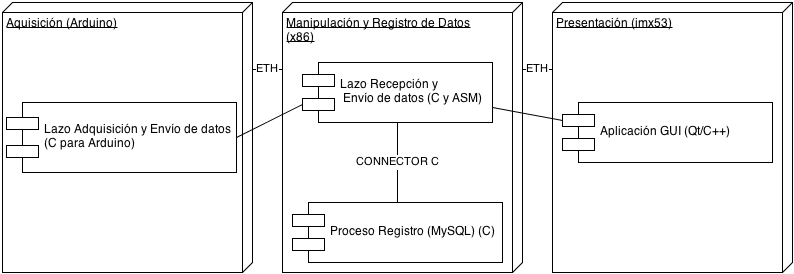
\includegraphics[width=1\textwidth,keepaspectratio=true]{img/Deployement.png}
  \caption{Diagrama de Despliegue del Sistema}
  \label{fig:esquema}
 \end{center}
\end{figure}

\subsection{\textcolor{orange}{Descripción del contexto del sistema}}

EL subsistema de Adquisición  de datos que se encuentra corriendo sobre una plataforma hardware arduino, envía datos de temperatura por medio de la interfaz Ethernet obtenidos mediante el instrumento adecuado para esto(sensor de temperatura),después de haberse identificado correctamente con el subsistema de manipulación y registro de datos el cual tendrá el rol de servidor sobre una plataforma hardware X86,donde se registran los datos de temperatura en una base de datos, mientras que el subsistema de presentación de datos que se encuentra corriendo en una plataforma hardware imx53 debidamente identificado con el servidor, es el encargado por medio de una conexión Ethernet, mostrar el dato de temperatura a través de un interfaz gráfica al usuario. 
Esta decisión de arquitectura se basa en el requerimiento funcional que especifica que el subsitema de de adquisición, registro, manipulación y presentación de datos  deben cumplir con una arquitectura Cliente-Servidor. 

\newpage

